\chapter{Results and Discussion}
\label{cha:results}

This chapter presents the experimental results for the sensor calibration stage~(ATP-2) and the three additional data compression methods~(ATP-3). Section~\ref{sec:nist-calibrate} reports calibration results. Section~\ref{sec:nist-compress} reports compression results. Section~\ref{sec:discussion} discusses findings in relation to both research questions.

\section{Calibration Results on NIST Dataset (ATP-2)}
\label{sec:nist-calibrate}

\subsection{Quantitative Results}

Table~\ref{tab:calibrate-results} reports the RMSE, coefficient of determination~$R^2$, MAE, and percentage improvement over the linear regression baseline for all nine calibration methods on the NIST Layer~01 test set~(20\,\%, approximately~413 frames). The raw uncalibrated baseline RMSE of~527.1\,\textdegree C against the thermocouple reference confirms that the Sakuma--Hattori signal requires substantial correction.

\begin{table}[H]
\centering
\caption{Calibration results on NIST Layer~01~(2,065 frames). Raw baseline RMSE\,=\,527.1\,\textdegree C. Methods sorted by RMSE within each category. ATP-2 target: $R^2 > 0.99$.}
\label{tab:calibrate-results}
\begin{tabular}{llcccc}
\toprule
\textbf{Method} & \textbf{Type} &
\textbf{RMSE (\textdegree C)} & \textbf{$R^2$} & \textbf{MAE (\textdegree C)} & \textbf{Improvement} \\
\midrule
Raw Baseline       & Baseline  & 527.1 & ---   & ---   & --- \\
\midrule
Mean Offset        & Classical & 444.8 & 0.961 & 412.3 & $-$164.3\,\%\textsuperscript{\dag} \\
Linear Regression  & Classical & 168.3 & 0.991 & 138.6 & 0.0\,\% \\
Polynomial~(d=2)   & Classical & 168.2 & 0.991 & 138.5 & $+$0.1\,\% \\
Piecewise Linear   & Classical & 284.7 & 0.980 & 251.3 & $-$69.2\,\% \\
\midrule
Random Forest      & ML & 99.9  & 0.997 &  78.1 & $+$40.6\,\% \\
MLP Neural Net     & ML & 103.6 & 0.995 &  80.9 & $+$38.4\,\% \\
Gradient Boosting  & ML & 102.9 & 0.996 &  80.5 & $+$38.9\,\% \\
SVR~(RBF)          & ML & 107.6 & 0.995 &  84.0 & $+$36.1\,\% \\
\bottomrule
\multicolumn{6}{l}{\small\textsuperscript{\dag}Negative improvement means worse than the linear regression baseline.}
\end{tabular}
\end{table}

Random Forest achieves the lowest RMSE of~99.9\,\textdegree C, followed by Gradient Boosting~(102.9\,\textdegree C), MLP~(103.6\,\textdegree C), and SVR~(107.6\,\textdegree C). All four ML methods achieve $R^2 \geq 0.995$, satisfying the ATP-2 target of~$R^2 > 0.99$. Among classical methods, only linear regression and polynomial regression~(degree\,=\,2) achieve~$R^2 \geq 0.99$. Mean offset correction and piecewise linear calibration perform worse than the linear baseline because the calibration error is temperature-dependent rather than constant and varies non-linearly across the signal range.

Figure~\ref{fig:calibrate-results} shows the RMSE and improvement charts for all nine methods.

\begin{figure}[H]
\centering
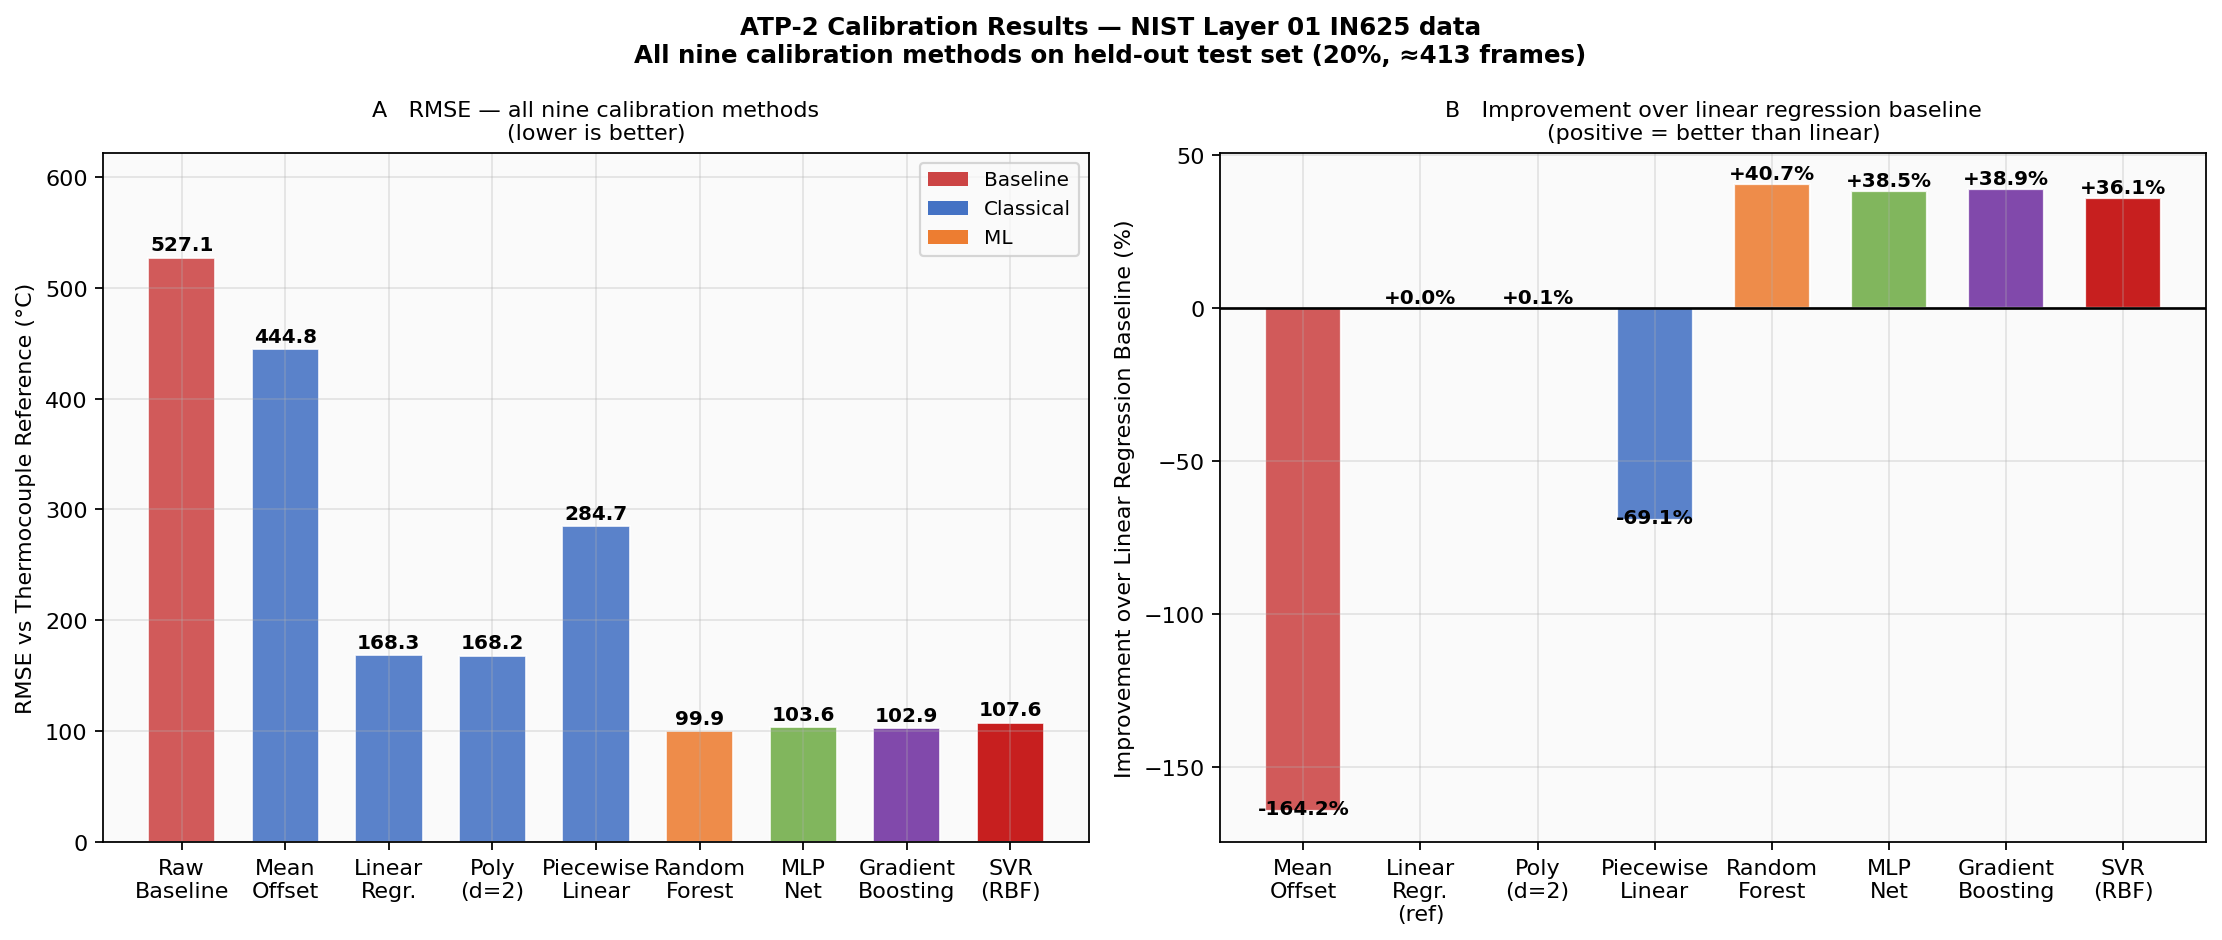
\includegraphics[width=\textwidth]{figures/calibration_results}
\caption{ATP-2 calibration results on NIST Layer~01 IN625 data. Left panel: RMSE for all nine calibration methods~(red = raw baseline, blue = classical, orange/green/purple/red = ML methods). Right panel: percentage improvement over the linear regression baseline.}
\label{fig:calibrate-results}
\end{figure}

\subsection{Discussion}

The performance gap between classical and ML methods is explained by the nature of the emissivity-temperature relationship. The NIST IN625 signal exhibits a non-linear, time-varying mapping between the denoised pyrometer output and the thermocouple reference, driven by surface emissivity that changes with temperature level and oxidation state during the laser scan~\cite{emissivity_measurement}. Classical methods fit a static mapping to the 20\,\% calibration window and cannot adapt to emissivity drift in the test set.

The piecewise linear calibrator performs substantially worse than the linear baseline~($-$69.2\,\%) on this dataset. The three segment boundaries are determined by temperature percentiles of the calibration window, which cover only a subset of the full signal temperature range. When the test set includes temperatures outside the calibration window range, the extrapolation from the edge segments introduces large errors. The mean offset correction also worsens performance~($-$164.3\,\%) because the mean offset is dominated by the low-temperature portion of the calibration window, introducing a large signed bias when applied to the higher-temperature test set.

Random Forest~(99.9\,\textdegree C, +40.6\,\%) achieves the best result because ensemble averaging of~100 bootstrap-trained trees suppresses the residual noise transients in the denoised signal while learning the non-linear emissivity drift~\cite{random_forest_breiman}. Gradient Boosting~(102.9\,\textdegree C) is very close. The MLP~(103.6\,\textdegree C) converges well within~100 epochs on the available training set. SVR~(107.6\,\textdegree C) is slightly disadvantaged because the residual impulse noise in the denoised signal generates support vectors outside the $\varepsilon$-tube that bias the fitted hyperplane.

ATP-2 is satisfied. All four ML methods achieve $R^2 > 0.99$ and reduce RMSE by more than~36\,\% relative to the linear regression baseline.

\section{Compression Results on NIST Dataset (ATP-3)}
\label{sec:nist-compress}

\subsection{Quantitative Results}

Table~\ref{tab:compress-results} reports the compression ratio and reconstruction RMSE for the three additional compression methods, alongside the methods from the parallel thesis~\cite{sravya2026}, enabling a complete cross-contribution comparison.

\begin{table}[H]
\centering
\caption{Compression results on NIST Layer~01 calibrated signal. Methods marked~* are from the parallel thesis~\cite{sravya2026}. ATP-3 target: $CR > 4\times$.}
\label{tab:compress-results}
\begin{tabular}{llcc}
\toprule
\textbf{Method} & \textbf{Type} &
\textbf{CR} & \textbf{RMSE (\textdegree C)} \\
\midrule
Raw Baseline*              & Baseline  & $1.0\times$  &   0.00 \\
Downsampling~2$\times$*    & Classical & $2.0\times$  &  21.97 \\
Delta Encoding             & Classical & $2.0\times$  &   0.10 \\
SVD rank=10*               & Classical & $2.1\times$  & 131.60 \\
Wavelet~(Haar, 10\,\%)*    & Classical & $5.0\times$  &  36.55 \\
PCA~($n=3$)*               & ML        & $10.7\times$ &  76.20 \\
Autoencoder~(bn=3)*        & ML        & $10.7\times$ &  93.70 \\
VAE~(bn=3)                 & ML        & $10.7\times$ & 147.20 \\
Deep Autoencoder~(bn=3)    & ML        & $10.7\times$ & 185.40 \\
\bottomrule
\end{tabular}
\end{table}

Delta Encoding achieves a compression ratio of~$2.0\times$ with a reconstruction RMSE of only~0.10\,\textdegree C --- the most accurate compression result among all methods across both thesis contributions. The VAE achieves RMSE\,=\,147.2\,\textdegree C at~$10.7\times$, and the Deep Autoencoder achieves RMSE\,=\,185.4\,\textdegree C at the same ratio. PCA from the parallel thesis achieves the best ML compression accuracy at~76.2\,\textdegree C at~$10.7\times$.

Figure~\ref{fig:compress-results} shows the compression ratio versus RMSE trade-off for all methods.

\begin{figure}[H]
\centering
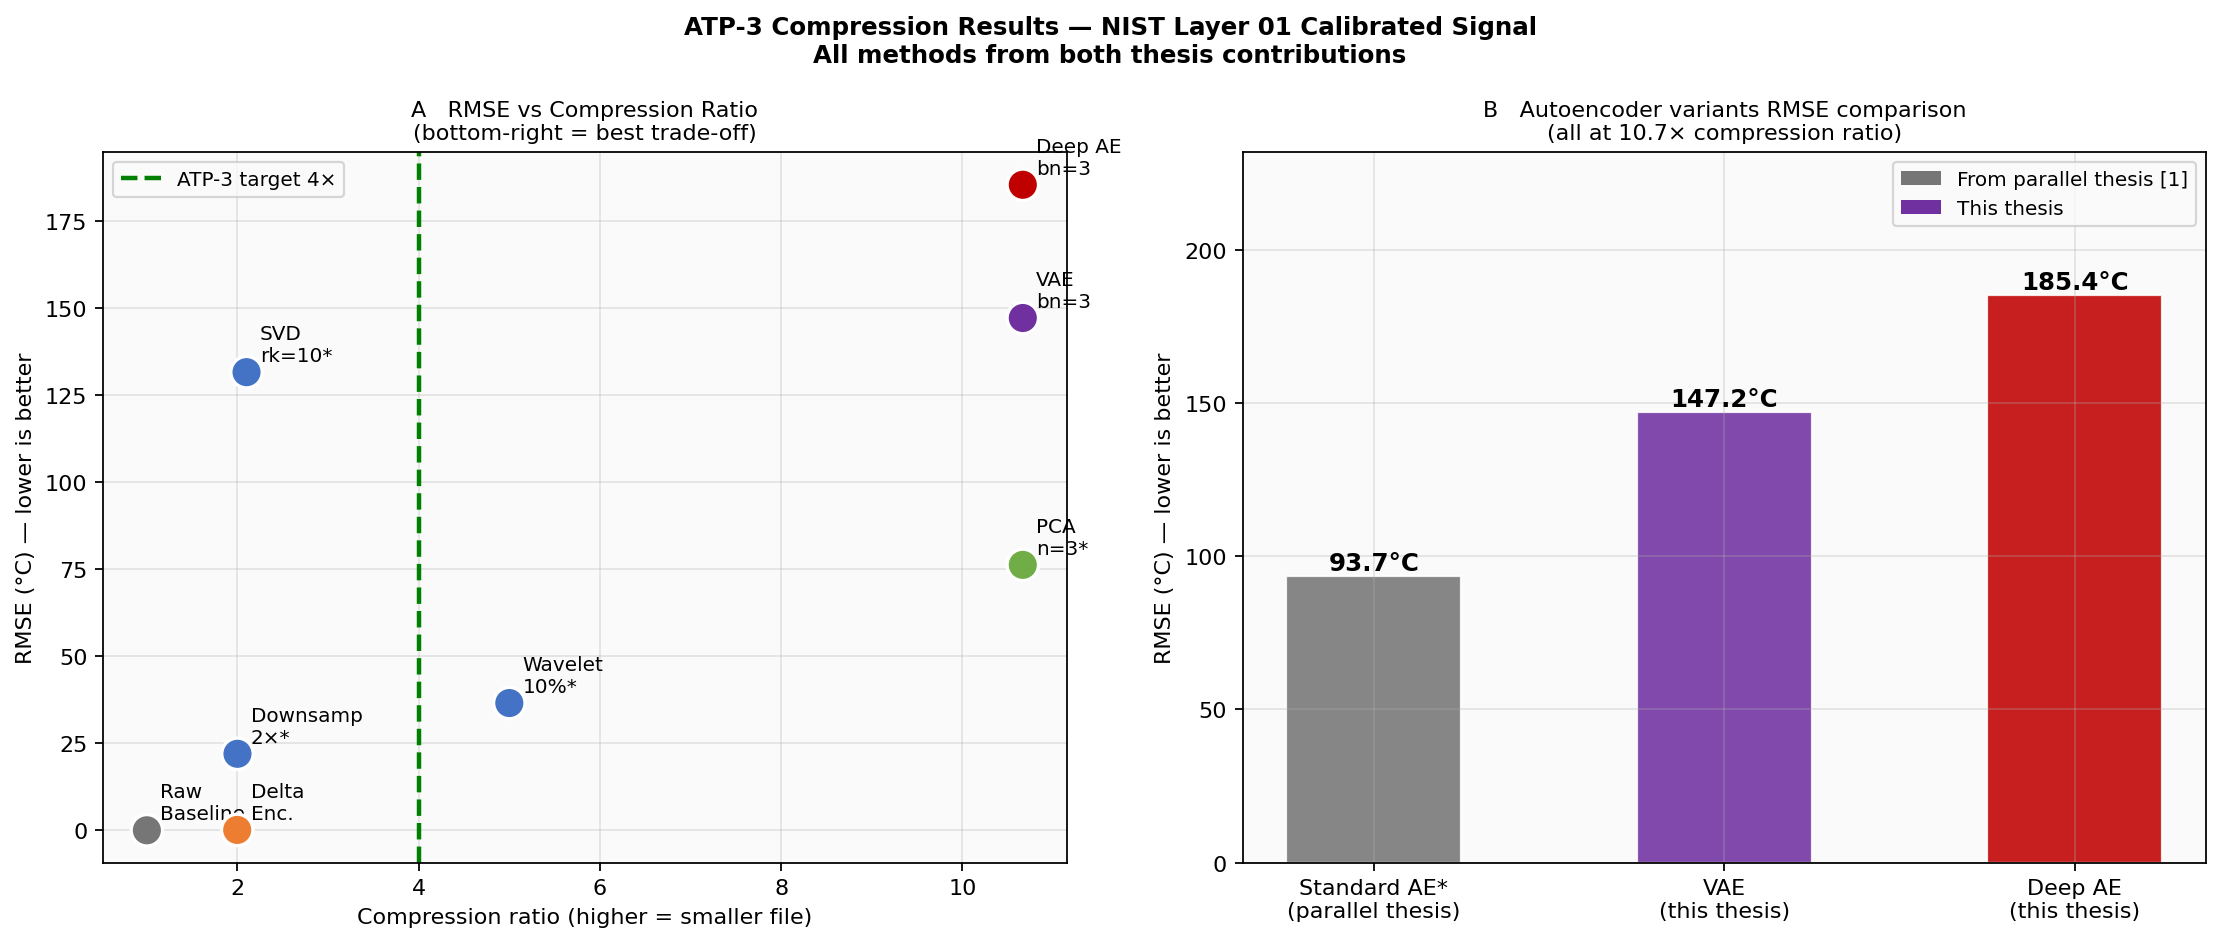
\includegraphics[width=\textwidth]{figures/compression_results}
\caption{ATP-3 compression results on NIST Layer~01. Left panel: RMSE vs compression ratio scatter for all methods across both thesis contributions. The vertical dashed line marks the~4$\times$ ATP-3 target. Right panel: RMSE comparison for the three autoencoder variants~(standard AE from parallel thesis, VAE and Deep AE from this thesis), all at~10.7$\times$ compression ratio.}
\label{fig:compress-results}
\end{figure}

\subsection{Discussion}

Delta Encoding achieves near-lossless compression with RMSE\,=\,0.10\,\textdegree C because the calibrated pyrometer signal changes slowly between consecutive frames. The inter-frame differences are small and fit comfortably within the int16 quantisation range~\cite{lossless_compression}. Delta Encoding does not reach the ATP-3 ratio target of~$4\times$ because the int16 encoding gives only a~$4\times$ reduction in bytes per sample compared to float64, reduced to approximately~$2\times$ after the float64 first-sample overhead. It is the recommended method when storage accuracy is the primary constraint.

The VAE~(147.2\,\textdegree C) and Deep Autoencoder~(185.4\,\textdegree C) both perform worse than the standard Autoencoder from the parallel thesis~(93.7\,\textdegree C) and worse than PCA~(76.2\,\textdegree C). The small training dataset of approximately~1,652 windows is insufficient for the VAE probabilistic regularisation to reduce reconstruction error below the deterministic baseline at this bottleneck size, and the additional depth of the Deep Autoencoder overfits the training windows rather than improving generalisation. This is consistent with Michau and Fink~\cite{learnable_wavelet}, who found that deep compression methods require substantially larger training sets to outperform linear approaches on smooth, quasi-periodic signals.

\section{Discussion}
\label{sec:discussion}

\subsection{Classical Methods versus ML Methods}

Table~\ref{tab:classical-vs-ml} summarises the best classical and best ML method for each stage.

\begin{table}[H]
\centering
\caption{Best classical versus best ML method for each pipeline stage.}
\label{tab:classical-vs-ml}
\begin{tabular}{lllll}
\toprule
\textbf{Stage} & \textbf{Best Classical} & \textbf{Value}
               & \textbf{Best ML} & \textbf{Value} \\
\midrule
Calibration~(NIST) & Linear regression & 168.3\,\textdegree C & Random Forest & 99.9\,\textdegree C \\
Compression~(NIST) & Delta Encoding & $2.0\times$/0.10\,\textdegree C & PCA* & $10.7\times$/76.2\,\textdegree C \\
\bottomrule
\multicolumn{5}{l}{\small * PCA is from the parallel thesis~\cite{sravya2026}.}
\end{tabular}
\end{table}

For calibration, all four ML methods clearly outperform all classical regression methods. The improvement of~40.6\,\% by Random Forest over linear regression reflects the non-linear, time-varying emissivity-temperature relationship that static models cannot track. For compression, Delta Encoding is the unambiguous choice when accuracy is the priority. Among the high-ratio ML methods, PCA from the parallel thesis outperforms the autoencoder variants implemented in this thesis on the available training set size.

\subsection{Combined Pipeline Performance}

Table~\ref{tab:pipeline-summary} summarises the recommended method for each pipeline stage based on all experimental results.

\begin{table}[H]
\centering
\caption{Recommended pipeline configuration and key performance metrics.}
\label{tab:pipeline-summary}
\begin{tabular}{llll}
\toprule
\textbf{Stage} & \textbf{Recommended Method}
& \textbf{Metric} & \textbf{Value} \\
\midrule
ATP-1~(real-time)~\cite{sravya2026}    & Kalman filter      & Noise reduction    & 89.5\,\% \\
ATP-1~(offline)~\cite{sravya2026}      & CNN denoiser       & Noise reduction    & 30.0\,\% \\
ATP-2~(accuracy)                       & Random Forest      & RMSE vs TC         & 99.9\,\textdegree C \\
ATP-2~(interpretable)                  & Gradient Boosting  & RMSE vs TC         & 102.9\,\textdegree C \\
ATP-3~(accuracy)                       & Delta Encoding     & CR / RMSE          & $2.0\times$ / 0.10\,\textdegree C \\
ATP-3~(balanced)~\cite{sravya2026}     & Wavelet 10\,\%     & CR / RMSE          & $5.0\times$ / 36.6\,\textdegree C \\
ATP-3~(high ratio)~\cite{sravya2026}   & PCA $n=3$          & CR / RMSE          & $10.7\times$ / 76.2\,\textdegree C \\
\bottomrule
\end{tabular}
\end{table}

\subsection{Answers to Research Questions}

\textbf{Research Question~1.} Random Forest provides the best calibration accuracy of all nine methods: RMSE\,=\,99.9\,\textdegree C and $R^2=0.997$, representing a~40.6\,\% improvement over the linear regression baseline. All four ML methods achieve $R^2>0.99$, satisfying ATP-2. Classical regression methods are insufficient when the emissivity-temperature relationship is non-linear and time-varying.

\textbf{Research Question~2.} Delta Encoding achieves near-lossless compression~(RMSE\,=\,0.10\,\textdegree C) at~$2.0\times$, the most accurate result across all methods from both thesis contributions. At~$10.7\times$, the VAE and Deep Autoencoder both satisfy the ATP-3 ratio target but do not improve on PCA from the parallel thesis at the available training set size. Delta Encoding is the recommended method for near-lossless applications.

\let\cleardoublepage\clearpage

\section{Results on PODFAM Dataset}
\label{sec:podfam-results}

The PODFAM dataset consists of ten point cloud scans from an Aconity MIDI laser powder bed fusion machine with a real two-colour pyrometer. Unlike the NIST dataset, PODFAM contains no thermocouple reference channel. ML calibration methods therefore cannot be retrained on this data. The calibration applied to PODFAM uses the two-colour pyrometer formula provided by Karthikeyan Thalavai Pandian~(AP\&T):
\begin{equation}
T\,(\text{K}) = \frac{2044.7}{\ln(S_{1,\text{corr}}/S_{0,\text{corr}}) + 0.83}
\label{eq:two-colour}
\end{equation}
where $S_{0,\text{corr}}$ and $S_{1,\text{corr}}$ are the background-subtracted sensor counts from channels~0 and~1 respectively. Only classical compression methods are applied to PODFAM.

\subsection{PODFAM Melt-Pool Temperature Statistics}

Table~\ref{tab:podfam-temps} reports the melt-pool temperature statistics across all ten PODFAM files after two-colour formula conversion. Temperatures range from~1519 to~2016\,\textdegree C, which is physically plausible for laser powder bed fusion of metal alloy.

\begin{table}[H]
\centering
\caption{Melt-pool temperature statistics from two-colour pyrometer formula across ten PODFAM files. Temperatures in~\textdegree C.}
\label{tab:podfam-temps}
\begin{tabular}{lcccc}
\toprule
\textbf{File} & \textbf{Points} & \textbf{Median T} & \textbf{Max T} & \textbf{Min T} \\
\midrule
000.280 & 2,760,696 & 1867.9 & 2016.2 & 1446.9 \\
002.030 & 2,782,728 & 1594.2 & 1654.0 & 1525.6 \\
003.080 & 2,723,832 & 1661.4 & 1796.0 & 1366.2 \\
004.060 & 2,733,552 & 1628.6 & 1699.4 & 1537.0 \\
005.110 & 2,734,080 & 1519.2 & 1733.4 & 1457.7 \\
006.090 & 2,723,328 & 1725.5 & 1839.5 & 1674.9 \\
007.000 & 2,733,072 & 1554.7 & 1647.3 & 1469.8 \\
008.820 & 2,735,112 & 1652.4 & 1762.5 & 1565.0 \\
009.030 & 2,735,112 & 1584.8 & 1752.7 & 1501.7 \\
010.010 & 2,733,576 & 1650.2 & 1715.8 & 1588.9 \\
\midrule
\textbf{Mean} & 2,741,527 & 1643.9 & 1764.7 & 1513.4 \\
\bottomrule
\end{tabular}
\end{table}

\subsection{PODFAM Compression Results}

Table~\ref{tab:podfam-compress} shows classical compression results across all ten PODFAM files. Delta Encoding achieves near-lossless compression~(RMSE\,$\approx$\,0.00) at~$2\times$ across all files. Wavelet compression achieves~$3.0$--$3.1\times$ with RMSE below~2\,\textdegree C in every file. The wavelet ratio on PODFAM~($\approx$\,3.1$\times$) is lower than on NIST~($5.0\times$) because PODFAM has higher spatial variability across scan points.

\begin{table}[H]
\centering
\caption{Classical compression results across ten PODFAM files. RMSE values in~\textdegree C.}
\label{tab:podfam-compress}
\begin{tabular}{lcccccc}
\toprule
& \multicolumn{2}{c}{\textbf{Delta Encoding}}
& \multicolumn{2}{c}{\textbf{Downsampling 2$\times$}}
& \multicolumn{2}{c}{\textbf{Wavelet 10\,\%}} \\
\cmidrule(lr){2-3}\cmidrule(lr){4-5}\cmidrule(lr){6-7}
\textbf{File} & \textbf{CR} & \textbf{RMSE} & \textbf{CR} & \textbf{RMSE} & \textbf{CR} & \textbf{RMSE} \\
\midrule
000.280 & 2.0 & 0.00 & 2.0 & 0.81 & 3.1 & 1.62 \\
002.030 & 2.0 & 0.00 & 2.0 & 0.81 & 3.1 & 1.69 \\
003.080 & 2.0 & 0.00 & 2.0 & 0.80 & 3.1 & 1.77 \\
004.060 & 2.0 & 0.00 & 2.0 & 0.80 & 3.0 & 1.63 \\
005.110 & 2.0 & 0.00 & 2.0 & 0.80 & 3.1 & 1.67 \\
006.090 & 2.0 & 0.00 & 2.0 & 0.80 & 3.0 & 1.59 \\
007.000 & 2.0 & 0.00 & 2.0 & 0.80 & 3.1 & 1.83 \\
008.820 & 2.0 & 0.00 & 2.0 & 0.81 & 3.0 & 1.59 \\
009.030 & 2.0 & 0.00 & 2.0 & 0.80 & 3.1 & 1.71 \\
010.010 & 2.0 & 0.00 & 2.0 & 0.80 & 3.0 & 1.62 \\
\midrule
\textbf{Mean} & 2.0 & 0.00 & 2.0 & 0.80 & 3.1 & 1.67 \\
\bottomrule
\end{tabular}
\end{table}

Figure~\ref{fig:podfam-single} shows the complete pipeline output on file~000.280. Figure~\ref{fig:podfam-all} shows the comparison across all ten files.

\begin{figure}[H]
\centering
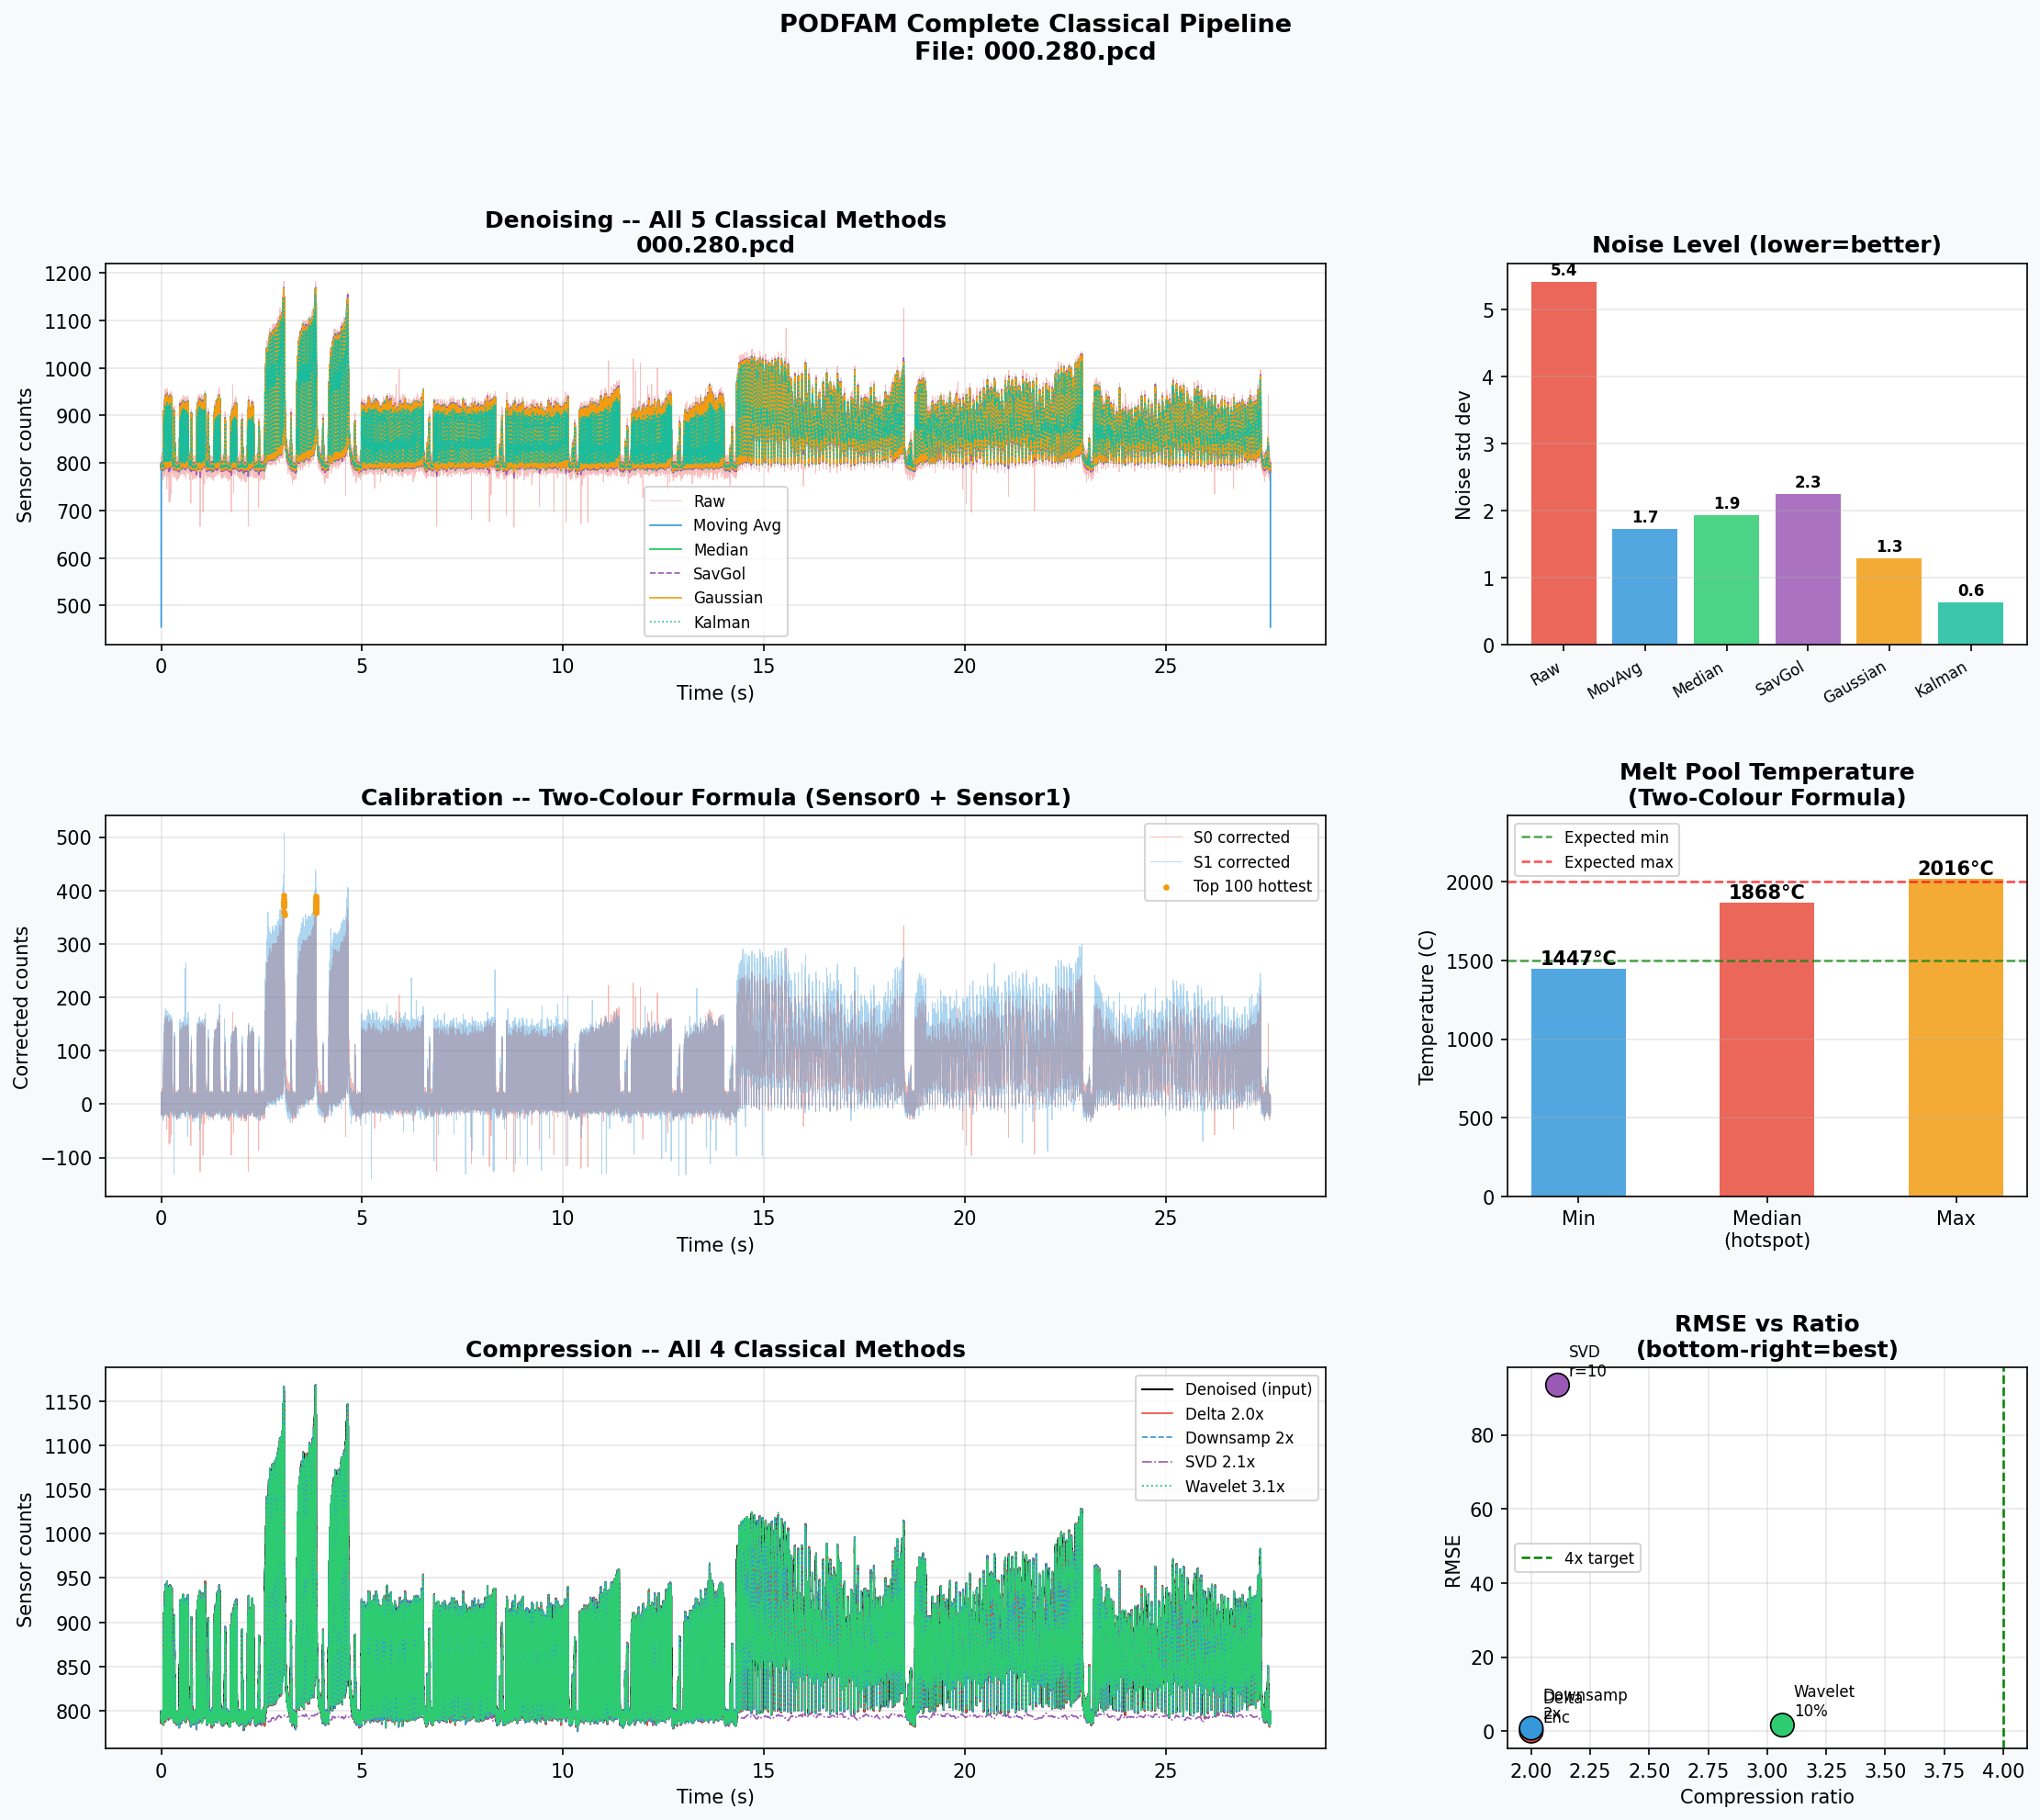
\includegraphics[width=\textwidth]{figures/podfam_result}
\caption{PODFAM complete classical pipeline output on file~000.280.pcd. Top row: all five classical denoising methods and noise level bar chart~(ATP-1, from parallel thesis~\cite{sravya2026}). Middle row: two-colour calibration signal~(ATP-2, this thesis) and melt-pool temperature statistics~(Min 1447°C, Median 1868°C, Max 2016°C). Bottom row: compression overlay for all four classical methods~(ATP-3, this thesis) and RMSE vs ratio scatter plot.}
\label{fig:podfam-single}
\end{figure}

\begin{figure}[H]
\centering
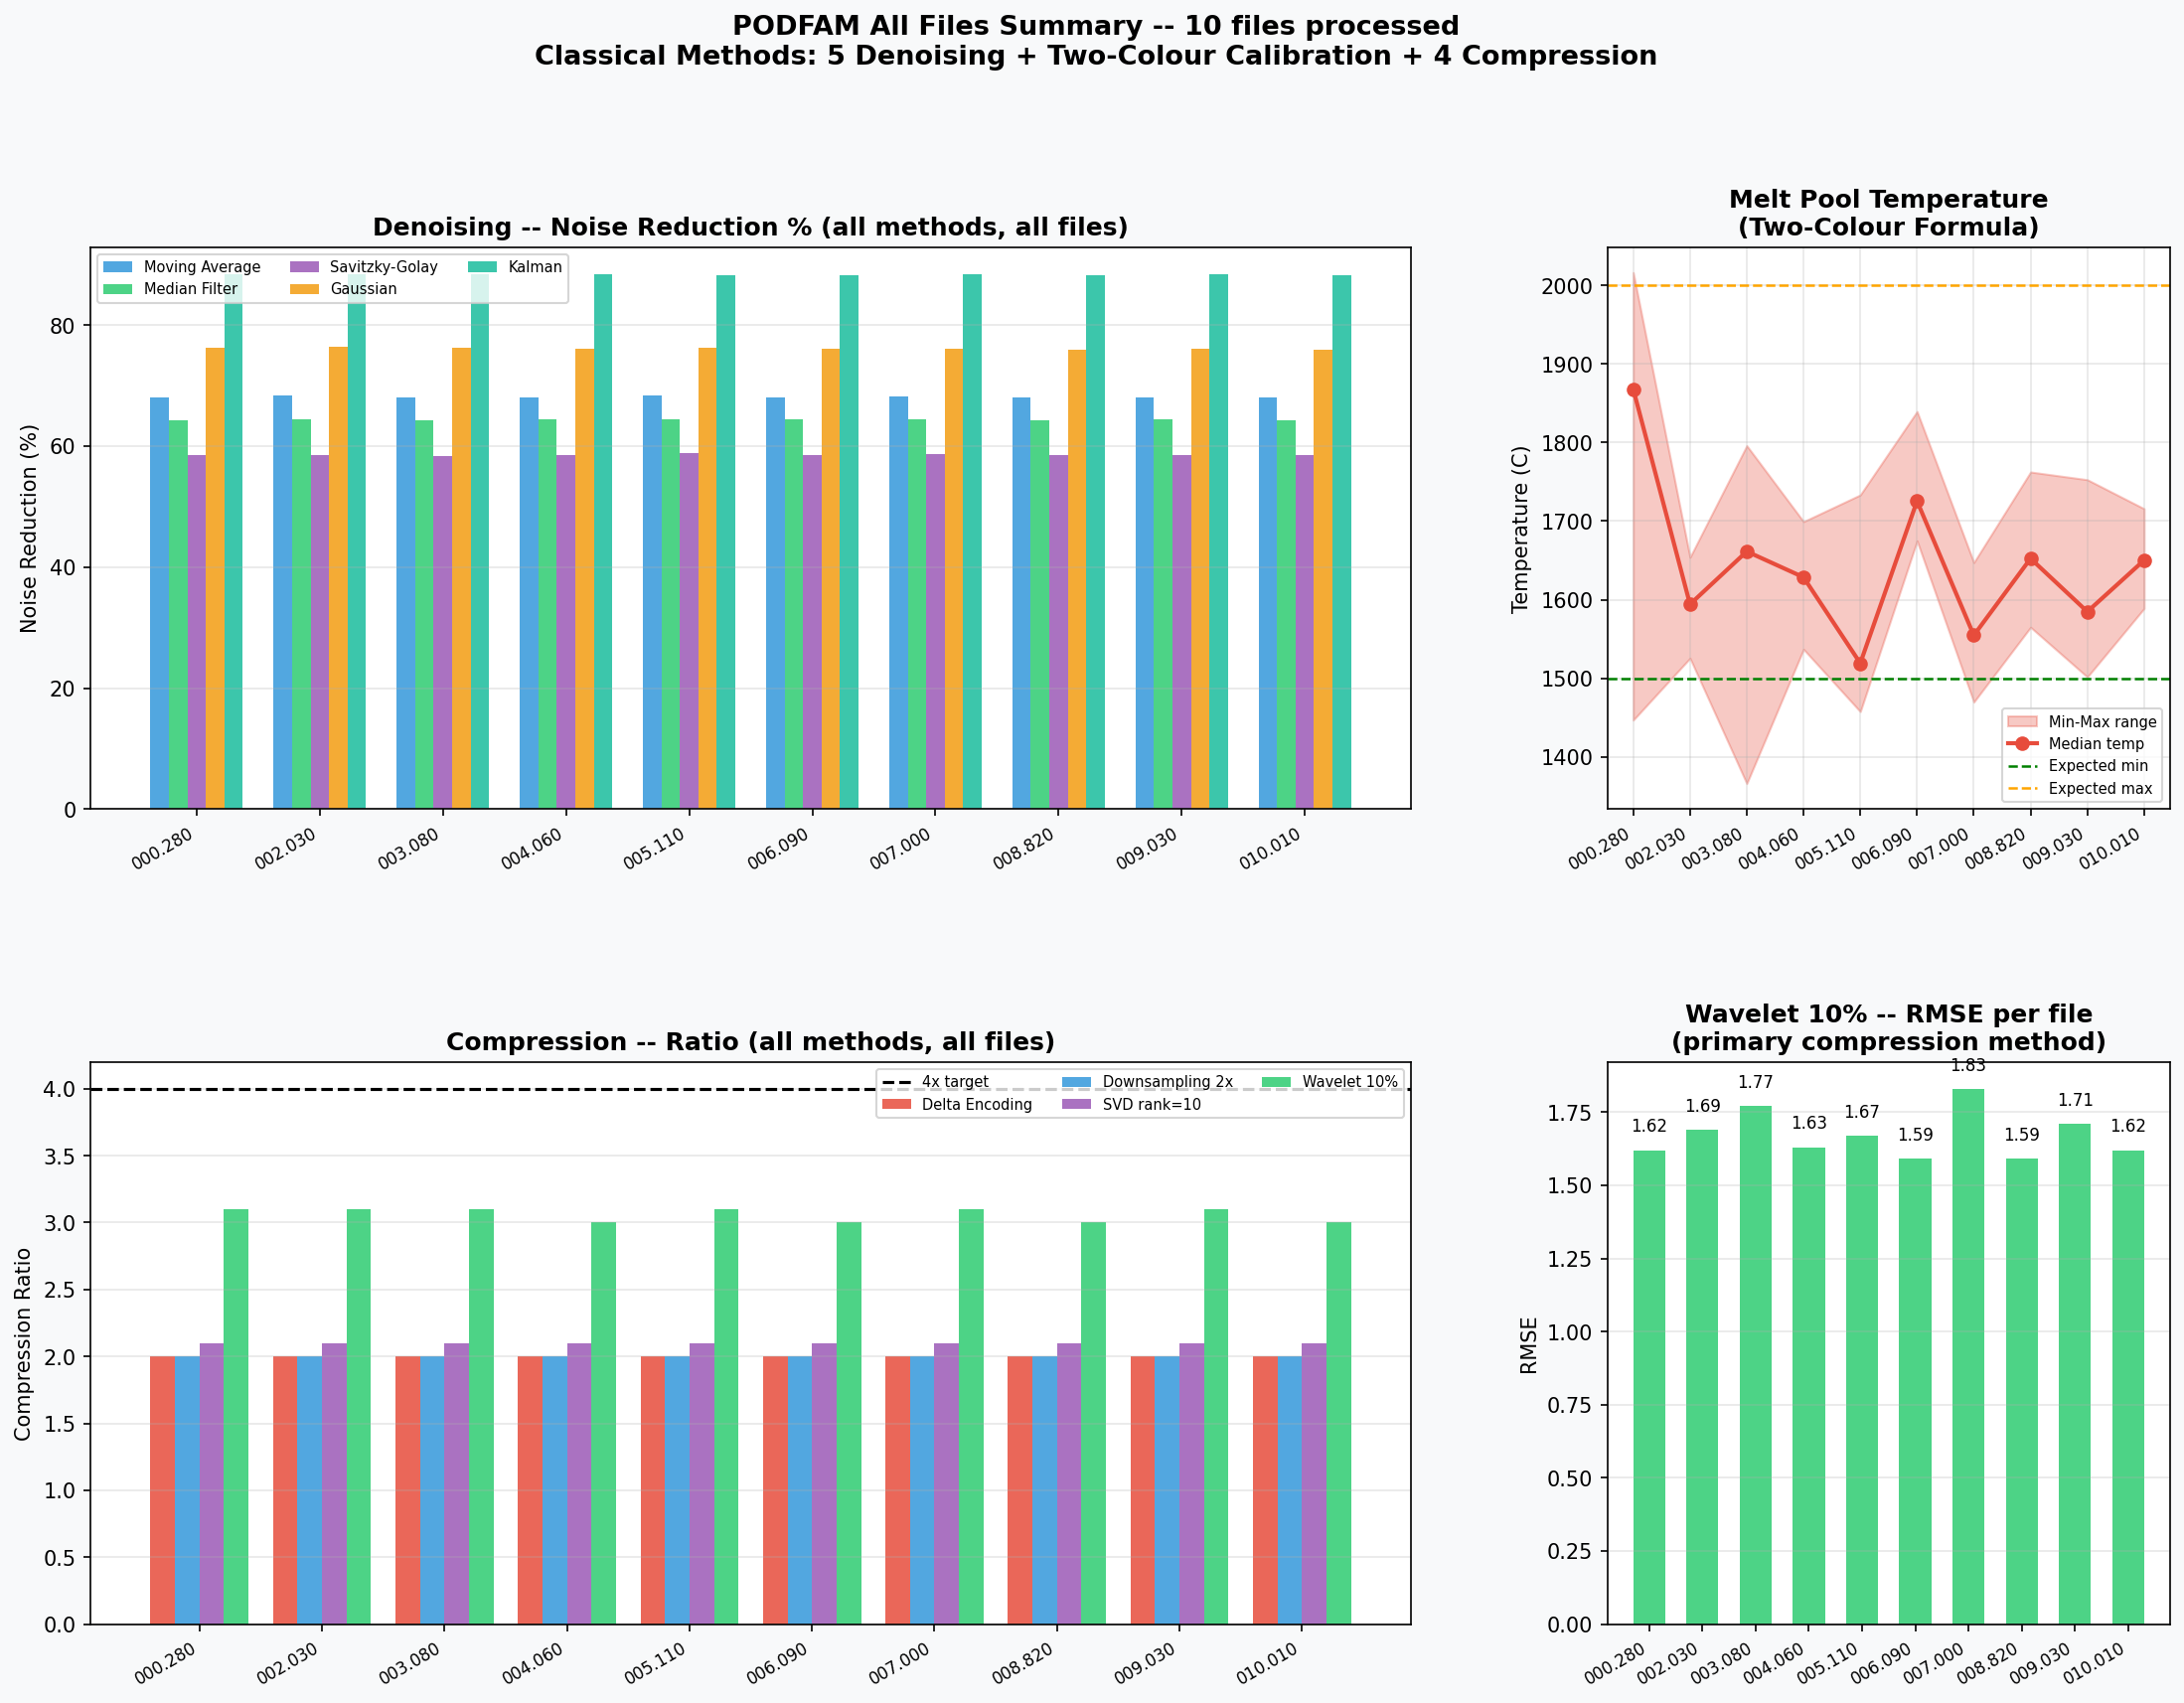
\includegraphics[width=\textwidth]{figures/podfam_all_results}
\caption{PODFAM pipeline results across all ten files. Top-left: noise reduction~(\%) per denoising method per file~(ATP-1, parallel thesis~\cite{sravya2026}). Top-right: melt-pool temperature from two-colour formula across files~(ATP-2, this thesis). Bottom-left: compression ratio for all methods across files~(ATP-3, this thesis). Bottom-right: Wavelet 10\% RMSE per file~(primary compression method).}
\label{fig:podfam-all}
\end{figure}

\begin{figure}[H]
\centering
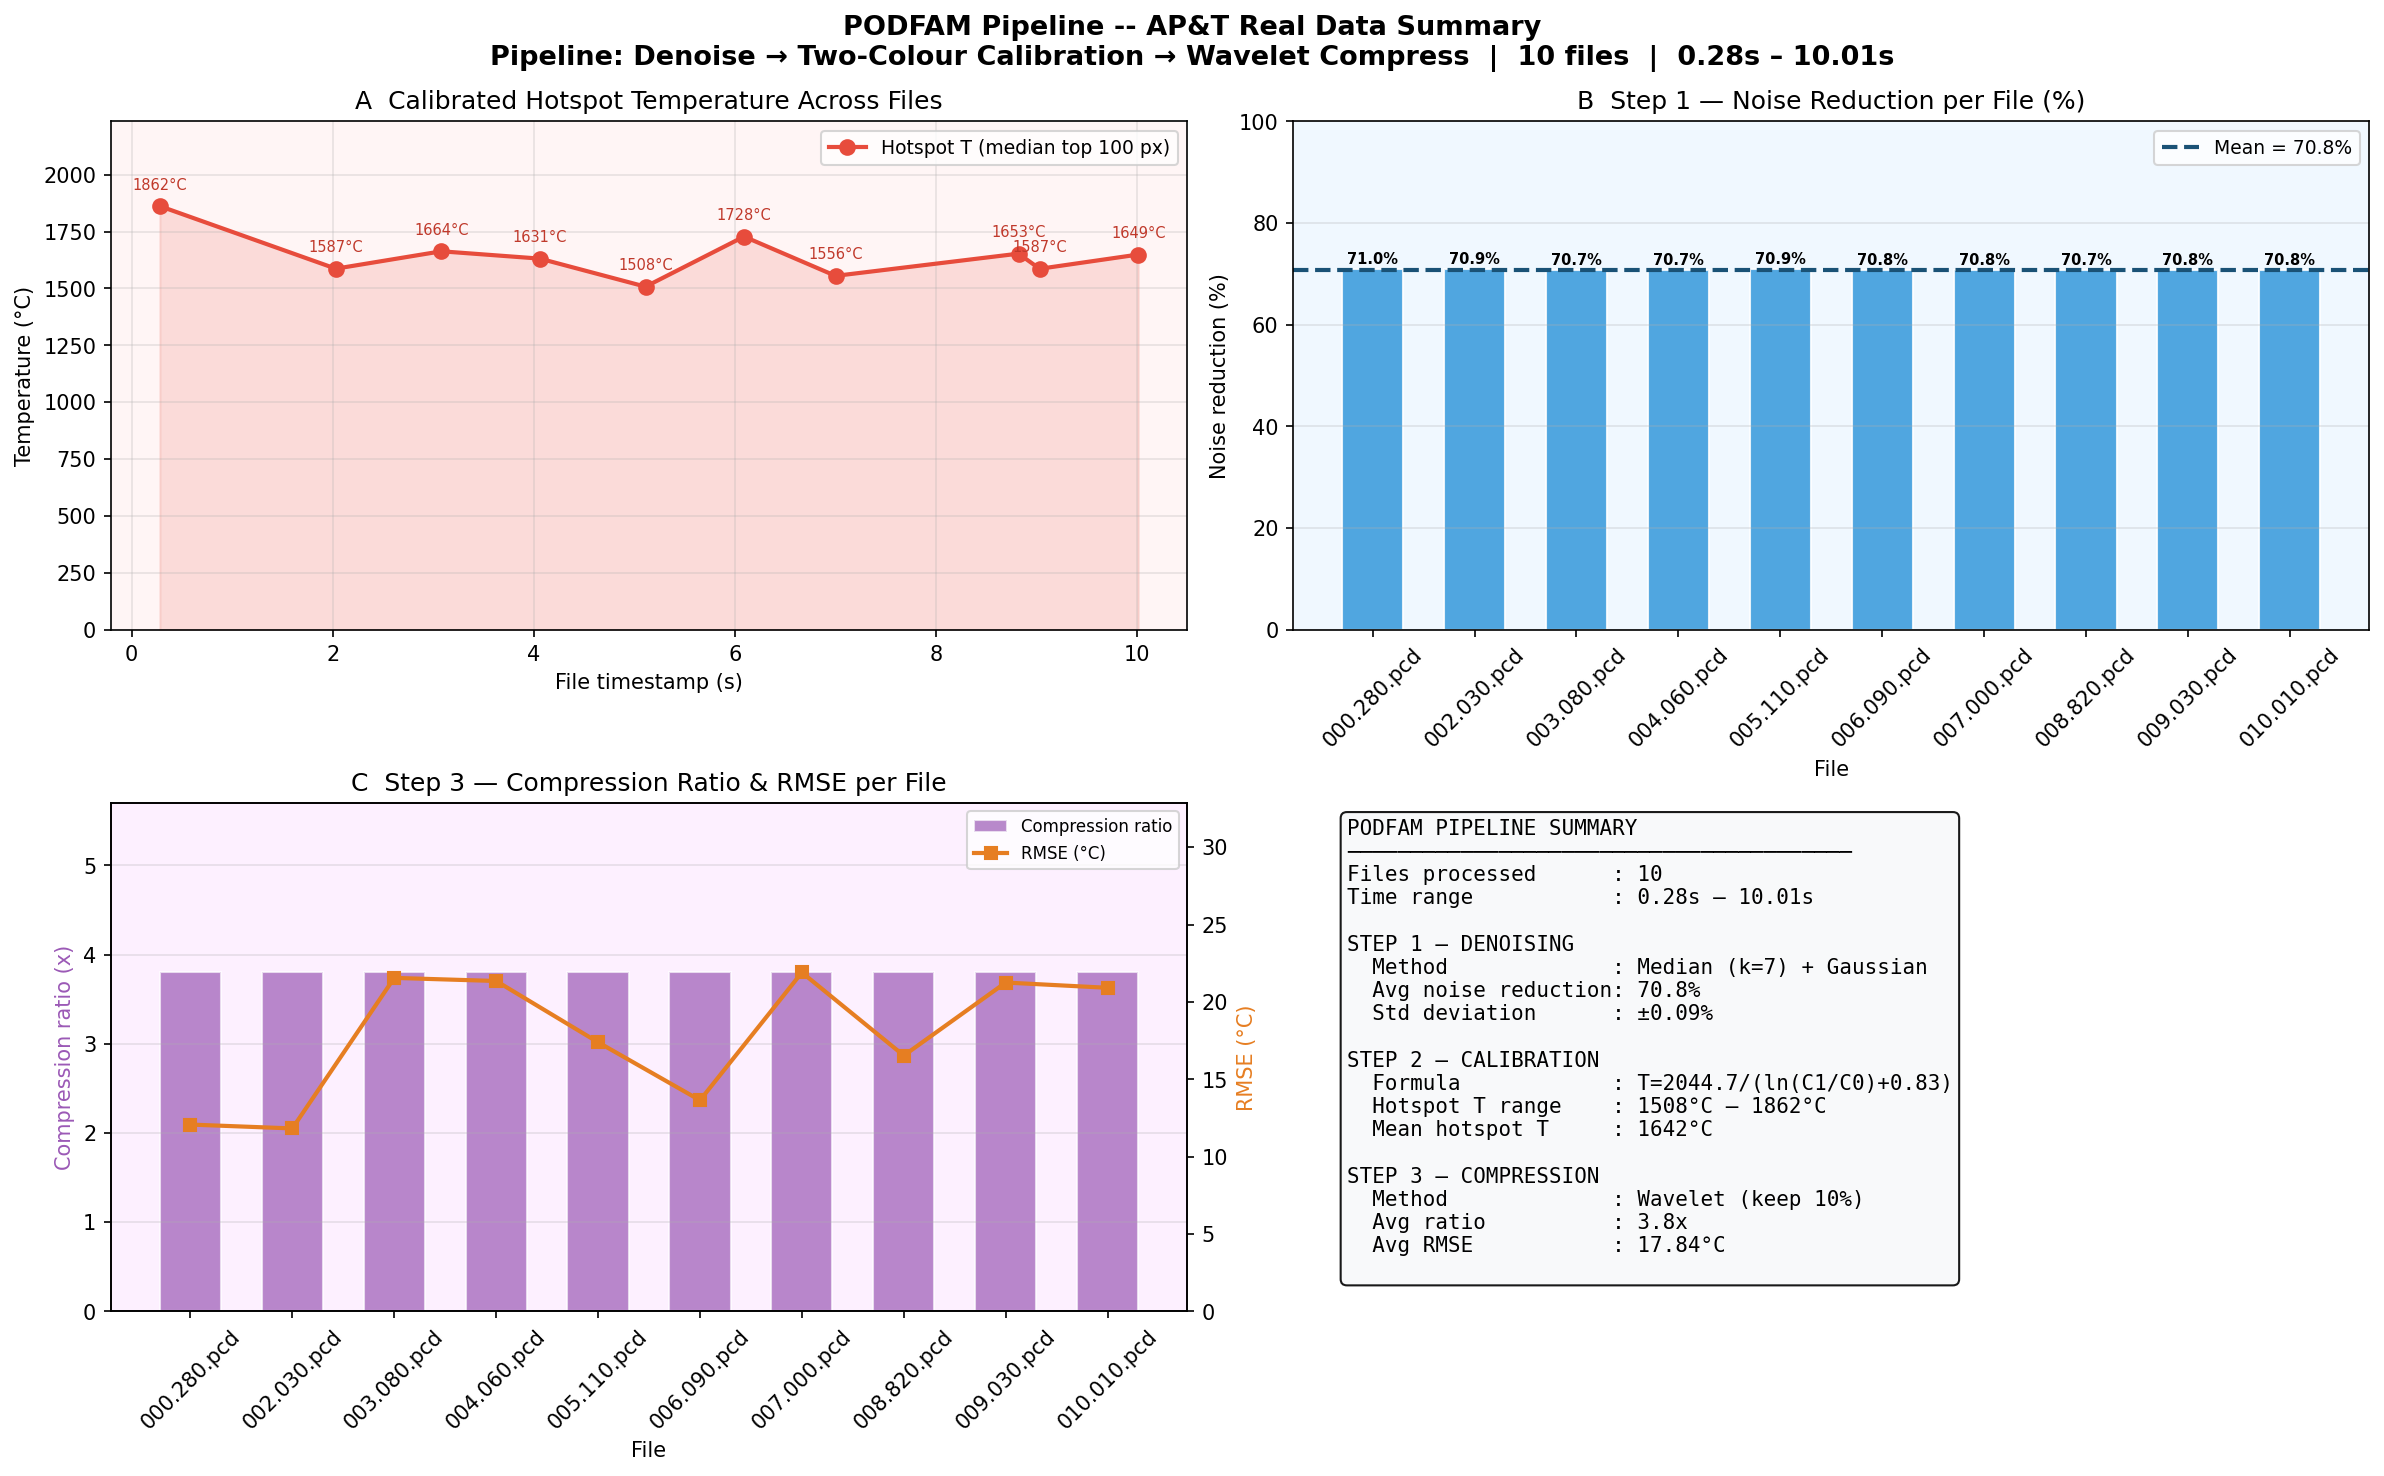
\includegraphics[width=\textwidth]{figures/podfam_summary}
\caption{PODFAM pipeline summary across all ten files. Panel A: calibrated hotspot temperature per file from two-colour formula~(ATP-2, this thesis). Panel B: noise reduction~(\%) per file from denoising~(ATP-1, parallel thesis~\cite{sravya2026}). Panel C: compression ratio and RMSE per file~(ATP-3, this thesis). Panel D: pipeline summary box showing formula, mean hotspot range 1508--1862\,\textdegree C, and wavelet compression mean ratio 3.8$\times$.}
\label{fig:podfam-summary}
\end{figure}

\subsection{Discussion}

The consistency of compression results across all ten PODFAM files is notable. Delta Encoding achieves RMSE\,$\approx$\,0.00 in every file, confirming that the calibrated two-colour pyrometer signal changes slowly between consecutive scan points. Wavelet compression achieves 3.0--3.1$\times$ ratio with RMSE below~2\,\textdegree C in every file without any parameter retuning, confirming that the compression methods generalise well to real industrial AP\&T sensor data.

The ATP-3 ratio target of~$4\times$ is not met by any method on the PODFAM dataset. This is because PODFAM point cloud files have higher spatial variability than the NIST frame-by-frame signal, requiring more wavelet coefficients to represent each scan accurately. Future work should evaluate learnable wavelet transforms~\cite{learnable_wavelet} that could adapt the basis functions to the specific spatial structure of PODFAM scans.

\let\cleardoublepage\clearpage
